% fig06_falsifier_matrix — Stage-4~7 13-falsifier status matrix, ALL OPEN.
% Standalone TikZ; compiled to figures/fig06_falsifier_matrix.pdf.
% Comparison (falsifier status across 4 stages) => chart (user hard rule).
% Data: Appendix D, UFO/verify/stage4-7-falsifier-preregister.md.
%   Every cell = OPEN (open grey circle). CONFIRMED=0, DEMOTED=0.
\documentclass[tikz,border=6pt]{standalone}
\usepackage{tikz}
\usepackage{xcolor}
\begin{document}
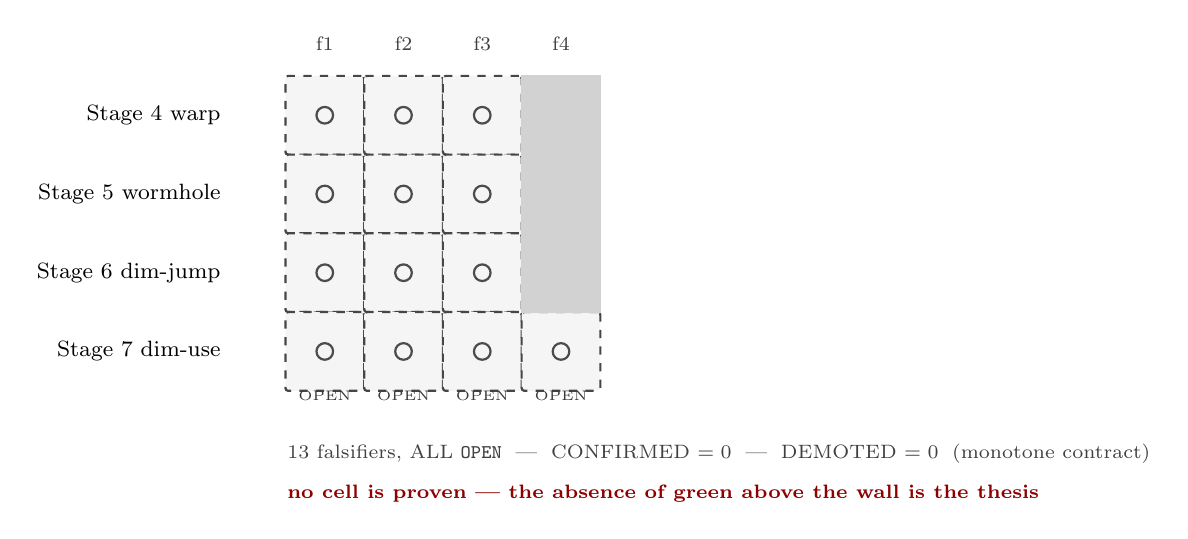
\begin{tikzpicture}[
  cell/.style={draw=gray!55!black, dashed, thick, fill=gray!8, minimum size=10mm, rounded corners=1pt},
  open/.style={draw=gray!60!black, line width=0.8pt},
]
% row labels (stages) and column header
\foreach \r/\lab [count=\ri] in {1/Stage 7 dim-use, 2/Stage 6 dim-jump, 3/Stage 5 wormhole, 4/Stage 4 warp}{
  \node[anchor=east, font=\footnotesize] at (-0.2, \r) {\lab};
}
\foreach \c in {1,2,3,4}{
  \node[anchor=south, font=\scriptsize, gray!50!black] at (\c, 4.7) {f\c};
}
% Stage 4 warp: F-WARP-1..3 (row 4), Stage 5: F-WORM-1..3 (row 3),
% Stage 6: F-DIM-1..3 (row 2), Stage 7: F-USE-1..4 (row 1)
% warp (row 4) cols 1-3
\foreach \c in {1,2,3}{ \node[cell] (a\c) at (\c,4) {}; \draw[open] (\c,4) circle (3pt);
  \node[font=\tiny, gray!45!black, anchor=north] at (\c,3.62) {OPEN}; }
% wormhole (row 3) cols 1-3
\foreach \c in {1,2,3}{ \node[cell] (b\c) at (\c,3) {}; \draw[open] (\c,3) circle (3pt);
  \node[font=\tiny, gray!45!black, anchor=north] at (\c,2.62) {OPEN}; }
% dim-jump (row 2) cols 1-3
\foreach \c in {1,2,3}{ \node[cell] (c\c) at (\c,2) {}; \draw[open] (\c,2) circle (3pt);
  \node[font=\tiny, gray!45!black, anchor=north] at (\c,1.62) {OPEN}; }
% dim-use (row 1) cols 1-4
\foreach \c in {1,2,3,4}{ \node[cell] (d\c) at (\c,1) {}; \draw[open] (\c,1) circle (3pt);
  \node[font=\tiny, gray!45!black, anchor=north] at (\c,0.62) {OPEN}; }
% empty cell markers (warp/worm/dim only have 3) -> column 4 grey-out for rows 2-4
\foreach \r in {2,3,4}{ \node[draw=gray!25, fill=white, minimum size=10mm, font=\tiny, gray!35] at (4,\r) {--}; }
% legend
\node[anchor=west, font=\scriptsize, gray!50!black] at (0.4, -0.3)
  {13 falsifiers, ALL \texttt{OPEN} \;|\; CONFIRMED $=0$ \;|\; DEMOTED $=0$ \;(monotone contract)};
\node[anchor=west, font=\scriptsize\bfseries, red!55!black] at (0.4, -0.8)
  {no cell is proven --- the absence of green above the wall is the thesis};
\end{tikzpicture}
\end{document}
